\documentclass[11pt]{article}
\usepackage[margin=0.85in,top=0.75in]{geometry}\usepackage[T1]{fontenc}\usepackage{lmodern}\usepackage{graphicx}
\usepackage{booktabs}\usepackage{amsmath}\usepackage[font=small,labelfont=bf]{caption}
\setlength{\parindent}{0pt}\setlength{\parskip}{0.42em}\pagestyle{empty}
\begin{document}
{\large\bfseries The Tell: Which Pitch-Sequencing Giveaways Survive New Games, and Whether Hitters Cash In}

\textbf{Introduction.} Advance scouts sell sequencing tells (``after a slider he doubles up''),
and clubs act on them in hitter meetings. No public method separates a real
tell from one found by searching hundreds of pitchers, counts and previous pitches. We ask how much
the previous pitch gives away beyond count and batter hand, how much of a scouted tell survives into
new games, whether hitters punish it, and whether the 2026 automated ball-strike (ABS) system
changed it.

\textbf{Methods.} We use all 2,049,352 regular-season Statcast pitches from 2024--2026 (1,793
pitcher-seasons with 250+ pitches). For each pitcher-season, nested models predict pitch type from
batter hand, then count, then the previous pitch, scored on games they never saw. The gain from the
previous pitch is TELL. A cue is the count, hand and previous pitch that most shifts one pitch
type's share. We find each pitcher's top cue in April--June (or 2025) and score it only on later
games. Whiff and run-value regressions hold pitcher-season, pitch type and count fixed. An in-season
alarm multiplies permutation e-values game by game. ABS is tested on paired pitchers against a
2024--25 placebo.

\textbf{Results.}
\begin{itemize}\setlength{\itemsep}{0.05em}\setlength{\topsep}{0.1em}
\item Added in that order, batter hand and count carry 102 and 58 millibits about the next pitch;
the previous pitch adds 8.1. A hitter guessing the likeliest pitch gains 0.6 points of accuracy on
average, and 5 against Dylan Cease.
\item Selection inflates tells. The top April--June cue shifts the next pitch by 26 points when found
and 10 points on July--September games, in the same direction 78\% of the time (no tell: 0 points,
50\%; Figure 1B). Across seasons, 28 points becomes 13.
\item The ten largest 2025 cues with enough 2026 data all kept their direction (Table 1).
\item TELL is reliable within a season (odd versus even games, 0.73) but not across seasons
($r = 0.19$, versus 0.62 for count usage).
\item Predictable pitches are not punished. From the 10th to the 90th percentile of predictability,
whiffs rise 0.6 points ($t = 4.7$) and run value improves 0.23 runs per 100 pitches ($t = 5.3$;
Figure 1C).
\item The alarm fired for 24\% of 2025 pitchers, at a median of 290 pitches (Figure 1D).
\item ABS lowered the top of the called zone by 1.2 inches (placebo 0.2) but moved TELL by
$-0.04$ millibits (95\% CI $-1.47$ to $+1.39$). The zone moved; sequencing did not.
\end{itemize}

\textbf{Conclusion.} Sequencing tells are real, season-specific, and less than half as large in new
games as when found. Scouts should discount them accordingly. Hitters show no sign of exploiting
them. The alarm gives clubs an in-season flag with a guaranteed false-alarm rate.
Code: \mbox{github.com/aidaneichman/the-tell}.

\begin{table}[h]\centering\small
\caption*{\textbf{Table 1.} Largest 2025 cues (50+ pitches; 25+ in 2026). Next-pitch share after the cue
versus otherwise (\%).}
\vspace{-0.4em}
\begin{tabular}{@{}lllcc@{}}\toprule
Pitcher & Situation & Next pitch & 2025 & 2026 \\\midrule
Dylan Lee & 0-1 vs RHB, after slider & slider & 75 vs 9 & 69 vs 25 \\
Jack Leiter & 1-2 vs LHB, after 4-seam & 4-seam & 22 vs 68 & 33 vs 50 \\
Kevin Gausman & 0-2 vs LHB, after 4-seam & 4-seam & 60 vs 15 & 51 vs 26 \\
Chris Sale & 0-1 vs RHB, after slider & 4-seam & 22 vs 66 & 30 vs 55 \\
Gregory Soto & 0-1 vs RHB, after sinker & sinker & 62 vs 19 & 46 vs 24 \\
Matthew Boyd & 2-2 vs RHB, after change & 4-seam & 71 vs 30 & 56 vs 28 \\
Hunter Brown & 0-1 vs RHB, after sinker & sinker & 62 vs 22 & 64 vs 28 \\
Kris Bubic & 1-0 vs RHB, after 4-seam & 4-seam & 54 vs 16 & 67 vs 24 \\
Drew Rasmussen & 1-2 vs LHB, after cutter & cutter & 7 vs 45 & 4 vs 30 \\
Dustin May & 1-2 vs LHB, after sweeper & sweeper & 31 vs 68 & 19 vs 42 \\
\bottomrule
\end{tabular}\end{table}

\begin{figure}[h]\centering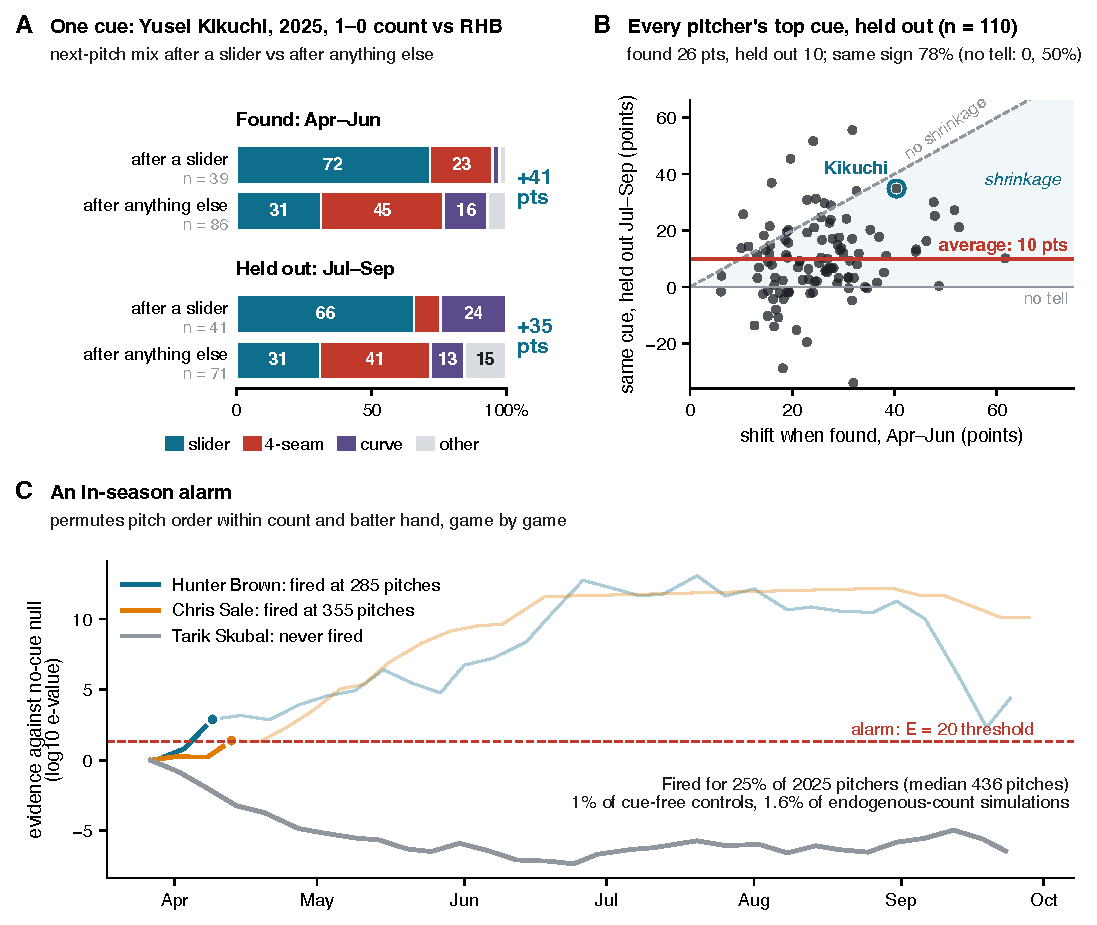
\includegraphics[width=\textwidth]{fig_abstract.pdf}
\caption*{\textbf{Figure 1.} (B) Cues with 30+ pitches each way. (C) Deciles, 95\% intervals. (D) Dots: alarm
fired.}
\end{figure}
\end{document}
